\subsection{Evaluating Machine Energy Efficiency and Performance using Control Charts}

In this section, it is discussed on how to use the energy baseline model to identify a benchmark reporting period, monitor EE and perform PDD. Building off of \cite{oakland_statistical_2008}, the choice of the benchmark reporting period in which the model is trained on is crucial as it provides a reference to which predictions are compared to. In \cite{cas}, the authors trained their MLR on a period of one year and plotted the instantaneous and cumulative residuals. These two SPC charts allowed the authors to analyze periods of \textit{best} CAS performance indicated by the residuals fluctuating around a mean of zero. Ultimately, the baseline model was then retrained on a time period of $36$ days representing the \textit{best} performance. Here, an example of a workflow for choosing the benchmark reporting period for the paper disposal machine is given.

Using the kernel design according to the evaluation metrics in Table \ref{tab:tab3}, the model is trained on $10$ minute aggregated data from October $11^{th}$ until October $15^{th}$. In Figure \ref{fig:fig14}, the top plot visualizes the instantaneous residuals of the in sample model fit, i.e., the difference of the predictions of the baseline model with the actual values of the benchmark reporting period. The bottom plot visualizes the cumulative residuals of the in sample fit. 

Where the SPC charts developed in this thesis differ from that in the literature and in industry is that the energy baseline model is a probabilistic model, and therefore, we have access to the uncertainty in our predictions. Where current SPC charts only take into account the point predictions and standard deviation of residuals to define UCL and LCL (as described in \hyperlink{subsection.2.3}{Section 2.3}), our proposed SPC charts utilizes the posterior distribution to define the control limits. Namely, by using the $95\%$ PI, a probabilistic approach can be used to determine the statistical significance of deviations in performance and change in EE over time. 

A red point in the top plot indicates that, at that time point $t$, the actual value was greater than $2 \sigma$ away from the mean prediction $\hat{\mu}_t$ and vice versa. Looking back at the time series plot in Figure \ref{fig:fig10}, one can potentially identify these outlier points. Then, in the CuSum plot, MA trend lines ($1$hr and $6$hr) are plotted to aid the identification of a benchmark reporting period. It can be seen that the slope of the residuals slightly increases until about the end of the day on October $12^{th}$, then is constant, and finally shows a slight decrease. However, in both charts, the mean of the residuals fluctuates around the zero bound, and thus the justification as using these four days for the benchmark reporting period is upheld.

\begin{figure}[h]
\centering
\graphicspath{ {./images/} }
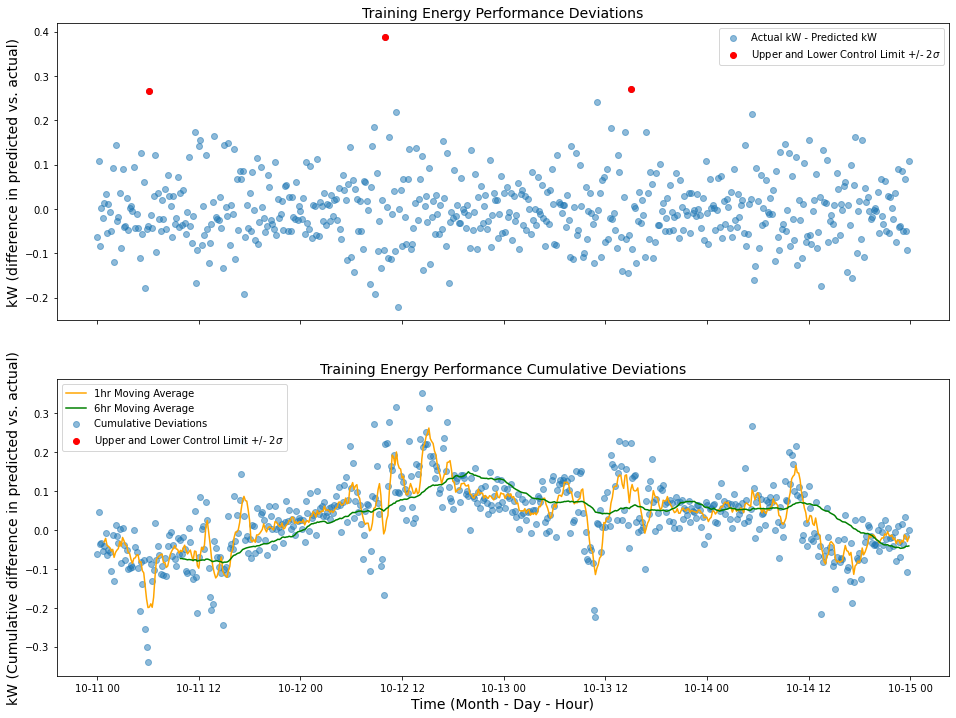
\includegraphics[scale=0.49]{images/entsorgung_baseline_SPC.png}
\caption{Benchmark reporting (training) period SPC charts.}
\label{fig:fig14}
\end{figure}

With a benchmark reporting period now chosen, predictions for every $10$ minutes for the next $24$ hours are computed. The same SPC charts are then visualized in Figure \ref{fig:fig15} as a hypothetical example to what the operators / production leaders may receive in a real production environment. In the top chart, around 10:30a.m the paper disposal machine was consuming much less energy than what was deemed plausible by the GP model. Indicated by the red dots, these values lie in succession and are $2\sigma$ away from the expected value. Subsequently, there is a reversion back to what seems to be the nominal operating conditions. The CuSum plot, indicated by the change in slope starting at about 8:30a.m until 11:45a.m, identifies this deviation as a large deviation in machine energy consumption. With the SPC charts having identified a change in EE as a result of a significant decrease in energy consumption, the original time series is plotted again in Figure \ref{fig:fig16}. Indeed, indicated by the red shading, there was a significant decrease in energy consumption. 

Furthermore, when a change in EE is identified, the time, machine, actual value, and degree of deviation (indicated by the z-score; how many standard deviations away a value is from the mean) is logged in a database where a historical registry of machine deviations can be built. Operations and maintenance teams can analyze this table to discuss each event, and the more data that is predicted and compared to the benchmark, the more valuable the registry becomes. For example, Figure \ref{fig:fig17} refers to the deviations that occurred on 15.10.2021, the type of machine, and the degree of deviation. To communicate z-scores to a non-technical audience, a color coding scheme is used where red indicates the actual value landed $3\sigma$ away, yellow is $2\sigma$, and green is $1\sigma$. The arrows indicate in which direction the deviation occurred, i.e., an energy decrease or increase.


\begin{figure}[h]
\centering
\graphicspath{ {./images/} }
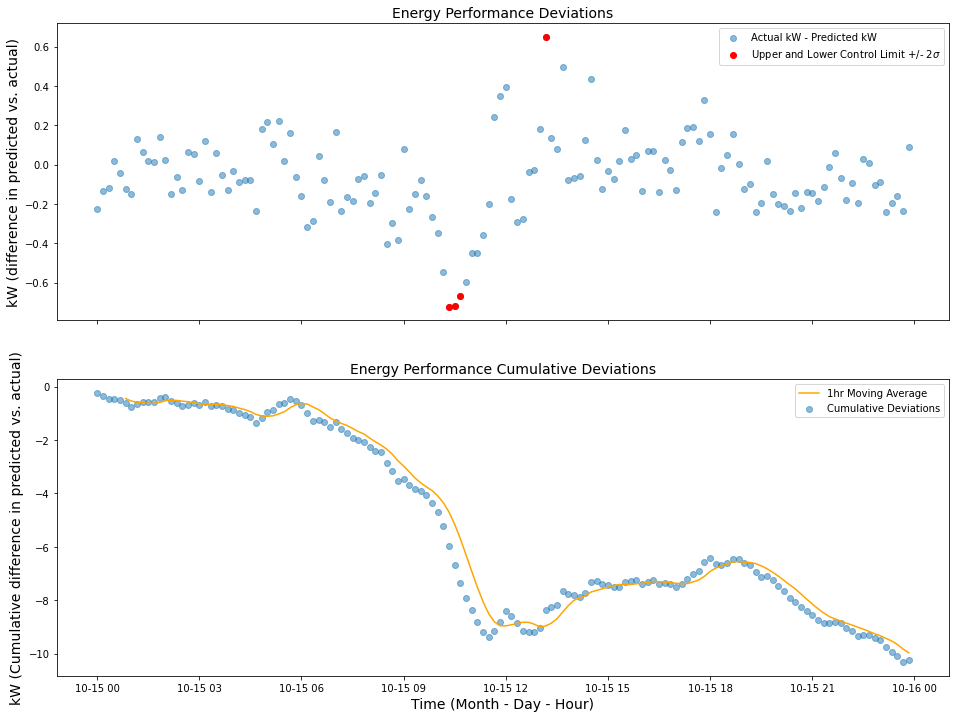
\includegraphics[scale=0.49]{images/entsorgung_test_SPC.png}
\caption{Using the test data, the paper disposal machine SPC charts are visualized. The top plot is the instantaneous residuals whereas the bottom is the CuSum of residuals.}
\label{fig:fig15}
\end{figure}

\begin{figure}[h]
\centering
\graphicspath{ {./images/} }
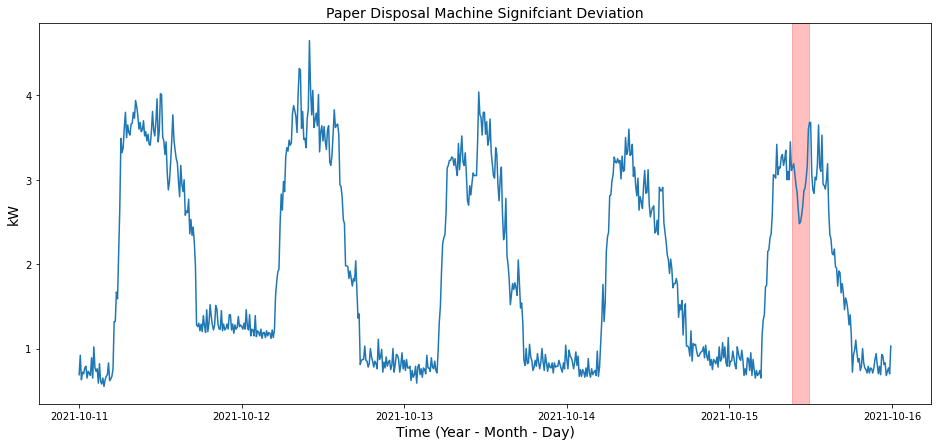
\includegraphics[scale=0.49]{images/entsorgung_deviation.png}
\caption{Original time series plotted for further analysis after the SPC charts and GP model identified a significant decrease in energy consumption indicated by the red shaded area.}
\label{fig:fig16}
\end{figure}

\begin{figure}[h]
\centering
\graphicspath{ {./images/} }
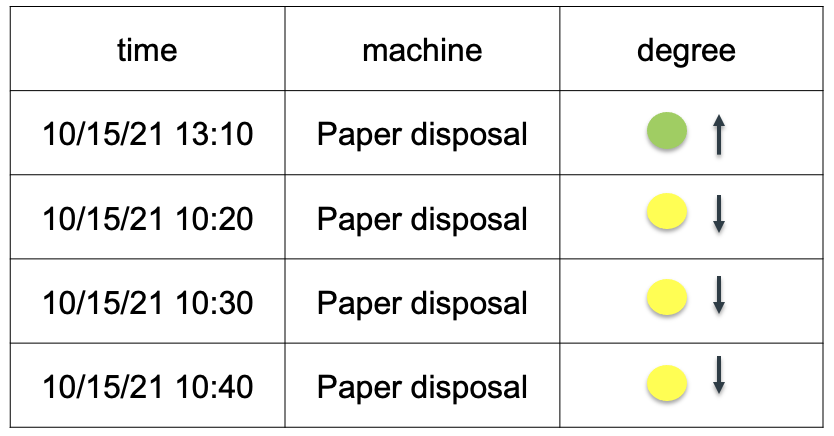
\includegraphics[scale=0.49]{images/entsorgung_registry.png}
\caption{Historical registry of paper disposal machine performance deviations. }
\label{fig:fig17}
\end{figure}

\subsection{Model Deployment Preparation}

Per the experimentation workflow in Figure \ref{fig:fig12}, the final step is to save the model's parameters (state) to a \path{.pth} file. Within this file is the full ``raw" state of the learned GPyTorch model parameters. Saving this to a file allows one to simply load the model's state back into an ExactGP module and perform inference without the need for any further training. To prepare the GPyTorch model for a prototype deployment in CLEMAP's environment and infrastructure, the focus will be on developing a Docker container for the \textit{inference} phase which consists only of the ExactGP module, model state, and kernel and data utilities.

Docker \footnote[3]{https://www.docker.com/} is an open source platform, free for personal use, that offers container technologies, lightweight alternatives to \ac{VM}, allowing applications to be deployed in independent, self-contained environments, matching the exact requirements of each model \cite{dreyfus-schmidt_introducing_2020}. Containerization of developed models is becoming a popular solution to the difficulties of dependencies when deploying machine learning models. Putting the inference phase into a container also allows for the orchestration of other containers in CLEMAP's environment. For example, their \ac{ETL} process is in a container, and by also having an inference container, these two can be orchestrated together such that the inference container is orchestrated (``runs") with the ETL container.

There are three main components to building a Docker container: (1) Dockerfile: a blueprint for building images, (2) Docker image: a template for running containers, and (3) Docker container: the container itself, which is the packaged piece of software / application. In the Dockerfile is a set of commands such as installation of python requirements from the \path{requirements.txt} file and which file to run. In the GitHub repository \cite{Stechschulte_Gaussian_Processes_for_2022}, this is the \path{__main__.py} file. After defining the Dockerfile, a Docker image, a lightweight standalone executable package of software that includes everything needed to run the application, is built. Upon successful building of the Docker image, the container can be ran, which will run the \path{__main__.py} file. As a final step, the Docker container is pushed to Docker Hub, a platform similar to GitHub where repositories can be created to manage containers, to be available for use by the CLEMAP team. 

\subsection{Assumptions and Limitations of Models}

One of the assumptions of the models is the benchmark reporting period. Ideally, one should have a longer time period to analyze and to choose this period from. Indeed, most of the related work in \hyperlink{section.2}{Section 2} had access to several months of data. The work conducted in this thesis was meant to be an exploration / proof of feasibility, and therefore access to more data was limited. A longer time series allows for a wider range of production processes and periodicity's to be modeled than the current production week implemented in this thesis.

In addition, a limitation of the current baseline model implementation is that it does not take into account other covariates or production processes. Rather, it is only an extrapolation based on the past. For example, a meeting with CLEMAP's client production leader on 12.05.2022 had stated the company plans the next week's production on the Thursday before. Therefore, there is the possibility to include the production as a covariate for some of the models. However, this information came too late in this thesis to incorporate. Furthermore, after speaking with the production leader, it is clear the production processes are complex and can vary from order to order. The heterogeneous production environment can make false positives more likely when changing production environments are not taken into account.